\subsection{Discrete Event Simulation in \omnet}
\label{sec:omnetpp}
Since most relevant literature we wish to build upon uses \omnet as their discrete event simulation framework some experiments were performed. The first goal of the experiments is to create a working installation of \omnet and create a development environment in which the proposed solution can be developed. The second goal is to get acquainted with the modelling language and framework. Lastly the experiments validate that the framework is suitable for performing experiments involving random processes.

\omnet is actively maintained, the latest version 6.0.1 was released on the 1st of September 2022. Several open-source projects building on top of \omnet exist such as INET\footnote{\url{https://github.com/inet-framework/inet}, accessed 5 December 2022} which is a collection of models for wired/wireless protocols ranging from the physical to the application layer. Recently (May 2022) INET has added support for several TSN standards.

After installing \omnet and creating a development environment the \omnet tutorial~\cite{omnettutorial} was followed. This tutorial consists of 18 exercises showing the different aspects of the NED language and framework. To further study the framework and asses the suitability of \omnet for experiments of random processes an assignment from the Embedded Systems course 2IMN25 - Quantitative Evaluation of Embedded Systems is performed again. During the course a theoretical model for the expected steady-state distribution of the number of items in an $M/M/1/K$ queue was made, let $x$ be the number of items in the system, $k$ the maximum number of items in the system, $\lambda$ the arrival rate of items and $\mu$ the service rate of the items, then for $0 \leq x\leq k$ the probability of finding $x$ items in the system is described using Equation~\ref{eq:mm1k}. 
\begin{equation}
    \label{eq:mm1k}
p_\infty (x) = \left(\frac{\lambda}{\mu}\right)^x\cdot\frac{1-\frac{\lambda}{\mu}}{1-\left(\frac{\lambda}{\mu}\right)^{k+1}}
\end{equation}

A model of an $M/M/1/K$ queueing system was made in \omnet which is visualized in Figure~\ref{fig:mm1k_sim}. The system consists of an \textit{entityGenerator} which creates items with an intergeneration time that is drawn from an exponential distribution with a configurable rate $\lambda$. The generated items are then stored in a \textit{queue} of configurable size $K$. The \textit{sink} component takes an item from the \textit{queue} and takes execution time to handle the item before discarding it. The execution time is also drawn from an exponential distribution with a configurable rate $\mu$. An experiment is set up in which we log the queue occupancy in the steady state, \omnet is configured to automatically log the queue occupancy, run a simulation for 800000 s of simulated time and discard the data from the warm-up period of 300000 seconds of simulated time. Because the queue occupancy data points from a single simulation are not independent of each other \omnet is configured to repeat the simulation 50 times with different seed values for the random distributions.

\begin{figure}[htbp]
    \centering
    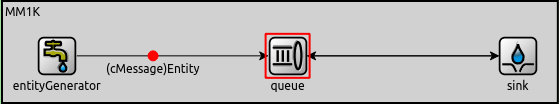
\includegraphics[width=\textwidth]{images/MM1K_sim.png}
    \caption{Visual view of an MM1K queue model in \omnet}
    \label{fig:mm1k_sim}
\end{figure}

The resulting data points are analysed with a python script in which we calculate the probability to find a certain queue occupancy in the simulation, with a 95\% confidence interval. The result of the simulation as well as the theoretical pdf are shown in Figure~\ref{fig:mm1k_sim}. The theoretical pdf falls inside the 95\% confidence interval for every queue occupancy, from this we conclude that the framework is able to properly simulate a random process.

\begin{figure}[htbp]
    \centering
    \includegraphics[width=\textwidth]{images/MM1k_analysis.png}
    \caption{Comparison of MM1K queue occupancy between simulation and theoretical analysis}
    \label{fig:MM1K_analysis}
\end{figure}

% \todo{write about logical modelling}

% \begin{figure}[htb]
%     \centering
%     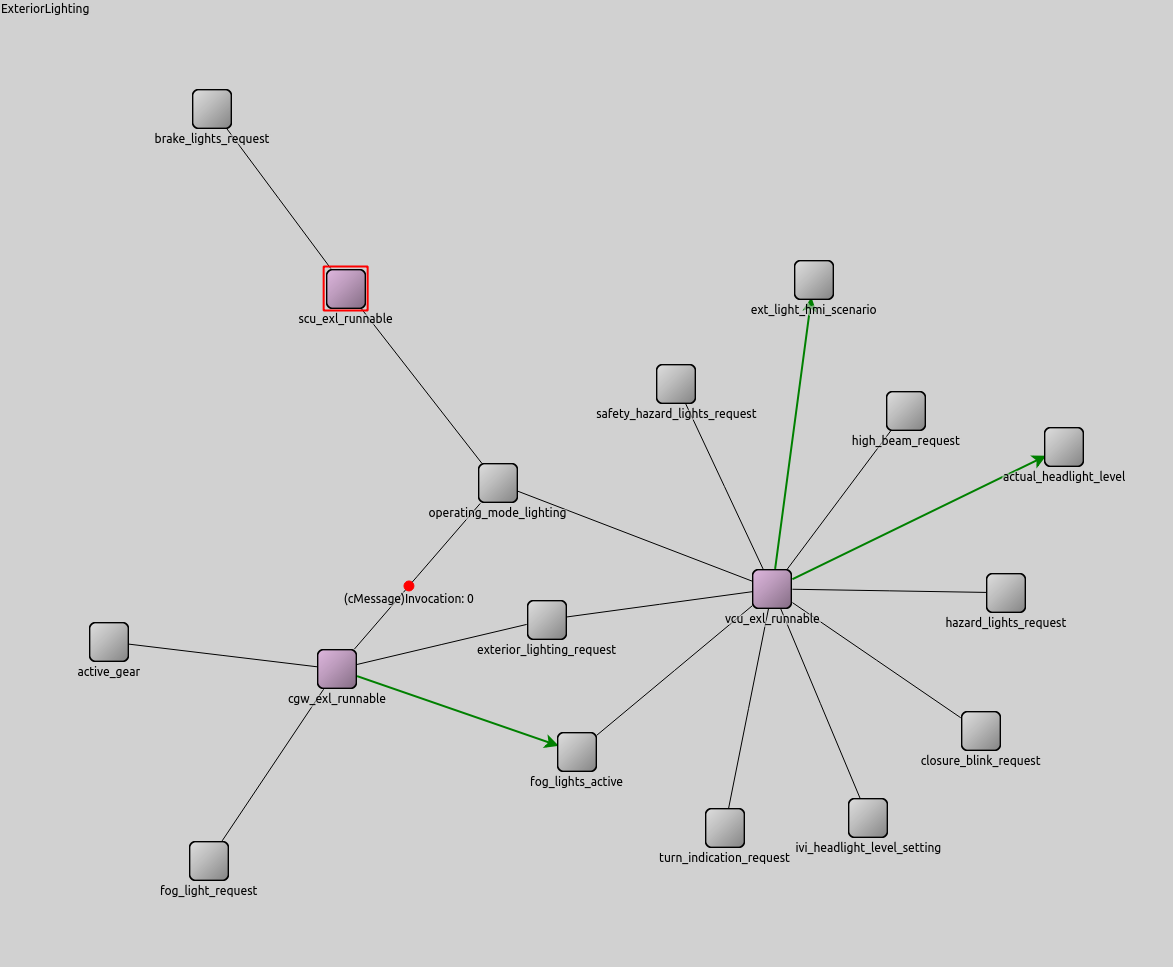
\includegraphics[width=\textwidth]{images/logical_sim.png}
%     \caption{Modelling signal transmission of the logical architecture in \omnet}
%     \label{fig:logical_sim}
% \end{figure}